\documentclass[a4, 12pt]{article}
\usepackage[a4paper, top=17mm, bottom=17mm, left=17mm, right=17mm]{geometry}
\usepackage[utf8]{inputenc}
\usepackage[T2A,T1]{fontenc}
\usepackage[colorlinks,filecolor=blue,citecolor=green,unicode,pdftex]{hyperref}
\usepackage{cmap}
\usepackage[english,russian]{babel}
\usepackage{amsmath}
\usepackage{amssymb,amsfonts,textcomp}
\usepackage{color}
\usepackage{array}
\usepackage{hhline}
\hypersetup{colorlinks=true, linkcolor=blue, citecolor=blue, filecolor=blue, urlcolor=blue, pdftitle=1, pdfauthor=, pdfsubject=, pdfkeywords=}
\usepackage[pdftex]{graphicx}
\usepackage{graphicx}
\usepackage{indentfirst}
\usepackage{multirow}
\usepackage{subfig}

\makeatletter
\bibliographystyle{utf8gost705u}	% Оформляем библиографию в соответствии с ГОСТ 7.0.5
\renewcommand{\@biblabel}[1]{#1.}	% Заменяем библиографию с квадратных скобок на точку:
\makeatother

\sloppy
\pagestyle{plain}

\title{Название статьи}

\author{Т.А.Брыксин \and Ю.В.Литвинов}
\date{}
\begin{document}

\maketitle
\thispagestyle{empty}

\begin{quote}
\small\noindent
Абстракт
\end{quote}

\section*{Введение}

Введение 

\section{Обзор}

Обзор~\cite{terekhov2009architecture}

\section{Основная часть}

\begin{figure} [ht]
  \begin{center}
    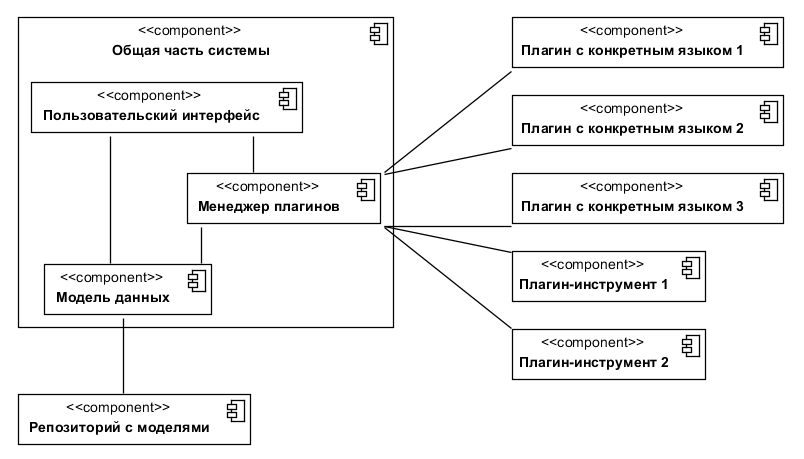
\includegraphics[width=0.9\textwidth]{fig1-architecture-overview.png}
    \caption{Картинка}
    \label{fig1}
  \end{center}
\end{figure}

\section*{Заключение}

Заключение

\nocite{*}

\addcontentsline{toc}{chapter}{\bibname}
\bibliography{biblio,ourWorks}

\end{document}
